\documentclass{article} % For LaTeX2e
\usepackage{iclr2020_conference,times}

% Optional math commands from https://github.com/goodfeli/dlbook_notation.
%\input{math_commands.tex}

\usepackage{hyperref}
\usepackage{url}


% added by FAFU

%\usepackage[utf8]{inputenc} % allow utf-8 input
%\usepackage[T1]{fontenc}    % use 8-bit T1 fonts
%\usepackage{hyperref}       % hyperlinks
%\usepackage{url}            % simple URL typesetting
%\usepackage{booktabs}       % professional-quality tables
%\usepackage{amsfonts}       % blackboard math symbols
%\usepackage{nicefrac}       % compact symbols for 1/2, etc.
%\usepackage{microtype}      % microtypography

% \usepackage[noabbrev,capitalize]{cleveref}
\usepackage{cleveref}
% \usepackage{caption}
% \usepackage[font=small]{caption}
\usepackage{subcaption}
% uncommented \input{math_commands.tex} for ICLR because then the following line caused an error
\newcommand{\ra}[1]{\renewcommand{\arraystretch}{#1}}
\usepackage{amsmath}
\usepackage{booktabs}
\usepackage{times}
%\usepackage[numbers]{natbib}
\usepackage{multicol}
\usepackage{graphicx}
% for tables side-by-side
\usepackage{geometry}
\usepackage{array, caption, floatrow, tabularx, makecell, booktabs}%
\captionsetup{labelfont = sc}
\setcellgapes{3pt}
\usepackage{mlmacros} % needs file mlmacros.sty
\usepackage[T1]{fontenc}
\usepackage[acronym,smallcaps,nowarn,section,nogroupskip,nonumberlist]{glossaries}
\renewcommand*{\glstextformat}[1]{\textcolor{black}{#1}}
\glsdisablehyper % disable hyperlinks to gls commands globally
\newacronym{VAE}{vae}{variational auto-encoder}
\newacronym{IS}{is}{importance sampling}
\newacronym{IWAE}{iwae}{importance-weighted auto-encoder}
\newacronym{FIVO}{fivo}{Filtering Variational Objectives}
\newacronym{SMC}{smc}{sequential Monte Carlo}
\newacronym{SSM}{ssm}{state-space model}
\newacronym{SGA}{sga}{stochastic gradient ascent}
\newacronym{SGD}{sgd}{stochastic gradient descent}
\newacronym{ELBO}{elbo}{evidence lower bound}
\newacronym{KL}{kl}{Kullback-Leibler}
\newacronym{LSTM}{lstm}{long short-term memory}
\newacronym{CNN}{cnn}{convolutional neural network}
\newacronym{MML}{mml}{maximum marginal likelihood}
\newacronym{NVIL}{nvil}{Neural Variational Inference and Learning}
\newacronym{VIMCO}{vimco}{Variational inference for Monte Carlo objectives}
\newacronym[firstplural=Imagination-Augmented Agent, plural=I2As]{I2A}{i2a}{imagination-augmented agent}

\newacronym{REINFORCE}{reinforce}{REINFORCE}
\glsunset{REINFORCE}
\newacronym{RL}{rl}{reinforcement learning}

\newacronym{ADAM}{adam}{ADAM}
\glsunset{ADAM}
\newacronym{RMSprop}{rmsprop}{RMSprop}
\glsunset{RMSprop}

\newacronym{GAN}{gan}{generative adversarial network}
\newacronym{GRU}{gru}{gated recurrent unit}
\newacronym{MLP}{mlp}{multilayer perceptron}
\newacronym{MC}{mc}{Monte Carlo}
\newacronym{bnp}{BNP}{Bayesian nonparametric}
\newacronym{mibp}{MIBP}{Markov Indian buffet process}
\newacronym{VRNN}{vrnn}{Variational Recurrent Neural Network}
\newacronym{LGSSM}{lgssm}{linear Gaussian state space model}
\newacronym[firstplural=recurrent neural networks, plural=RNNs]{RNN}{rnn}{recurrent neural network}

\newacronym{ELU}{elu}{exponential linear unit}

\newacronym{MNIST}{mnist}{mnist}
\glsunset{MNIST}

% HART and MOHART
\newacronym{HART}{hart}{hierarchical attentive recurrent tracking}
\newacronym{MOHART}{mohart}{multi-object hierarchical attentive recurrent tracking}

\newacronym{SOT}{sot}{single-object tracking}
\newacronym{MOT}{mot}{multi-object tracking}



% SQAIR
\newacronym{AIR}{air}{Attend, Infer, Repeat}
\newacronym{SQAIR}{sqair}{Sequential Attend, Infer, Repeat}
\newacronym{prop}{prop}{Propagation}
\newacronym{disc}{disc}{Discovery}

% SCA
\newacronym{MI}{mi}{mutual information}
\newacronym{CPC}{cpc}{contrastive predictive coding}
\newacronym{ICA}{ica}{independent component analysis}

\newacronym{CCR}{ccr}{capsule-camera-relationship}
\newacronym{CPR}{cpr}{capsule-part-relationship}
\newacronym{GMM}{gmm}{gaussian mixture model}
\newacronym{GQN}{gqn}{generative query network}
\newacronym{CCA}{cca}{Constellaton Capsule Autoencoder}
\newacronym{SCA}{sca}{Stacked Capsule Autoencoder}
\newacronym{ICAE}{icae}{Image Capsule Autoencoder}

\newacronym{OV}{ov}{object-viewer-relationship}
\newacronym{PV}{pv}{part-viewer-relationship}
\newacronym{OP}{op}{object-part-relationship}
\newacronym{SCAu}{scae}{Stacked Capsule Autoencoder}
\newacronym{PCAu}{pcae}{Part Capsule Autoencoder}
\newacronym{OCAu}{ocae}{Object Capsule Autoencoder}
\newacronym{CCAu}{ccae}{Constellation Capsule Autoencoder}

\newacronym[firstplural=degrees of freedom, plural=DoFs]{DOF}{dof}{degree of freedom}



% tighter bounds
\newacronym{AESMC}{aesmc}{auto-encoding sequential Monte Carlo}
\newacronym{PIWAE}{piwae}{partially importance-weighted auto-encoder}
\newacronym{MIWAE}{miwae}{multiply importance-weighted auto-encoder}
\newacronym{CIWAE}{ciwae}{combination importance-weighted auto-encoder}
\newacronym{AD}{ad}{automatic differentiation}
\newacronym{SPSA}{spsa}{simultaneous perturbation stochastic approximation}
\newacronym{CG-SPSA}{cg-spsa}{computational graph SPSA}
\newacronym{MAP}{map}{maximum a-posteriori}
\newacronym{KDE}{kde}{kernel density estimation}
\newacronym{EM}{em}{expectation maximization}
\newacronym{ALT}{alt}{alternating \textsc{elbo}s}
\newacronym{SNR}{snr}{signal-to-noise ratio}
\newacronym{MCM}{mcmc}{Markov Chain Monte Carlo}
\newacronym{RMSE}{rmse}{root mean squared error}


% rrws
\newacronym{SCFM}{scfm}{stochastic control-flow model}
\newacronym{WS}{ws}{wake-sleep}
\newacronym{BWS}{bws}{basic wake-sleep}
\newacronym{RWS}{rws}{reweighted wake-sleep}
\newacronym{WW}{ww}{wake-wake}
\newacronym{WWS}{wws}{wake-wake-sleep}
\newacronym{ESS}{ess}{effective sample size}
\newacronym{RELAX}{relax}{RELAX gradient estimator}
\newacronym{REBAR}{rebar}{REBAR gradient estimator}
\newacronym{PMF}{pmf}{probability mass function}
\newacronym{PCFG}{pcfg}{probabilistic context free grammar}
\renewcommand{\citep}[1]{(\citet{#1})}
\variables{a,g,t,x,y,z} % needs file mlmacros.sty

\newcommand{\opj}[1]{\textcolor{blue}{\textbf{opj}: #1}}
\newcommand{\OPJ}[1]{\todo{\opj{#1}}}

\newcommand{\ff}[1]{\textcolor{black}{\textbf{ff}: #1}}
\newcommand{\FF}[1]{\todo{\ff{#1}}}

% \usepackage{titlesec}

% \titlespacing*{\section}{0pt}{.1\baselineskip}{.1\baselineskip}
% \titlespacing*{\subsection}{0pt}{0.1\baselineskip}{0.1\baselineskip}

% \setlength\floatsep{0.1\baselineskip plus 3pt minus 2pt}
% \setlength\textfloatsep{1.\baselineskip plus 3pt minus 2pt}
% \setlength\intextsep{1.0\baselineskip plus 3pt minus 2 pt}

% \title{Permutation Invariance and \\ Relational Reasoning in Multi-Object Tracking}
% \title{Improving End-to-End Object Tracking Using\\Relational Reasoning}
\title{End-to-end Recurrent Multi-Object Tracking and Trajectory Prediction with Relational Reasoning}                                                                                             
% Authors must not appear in the submitted version. They should be hidden                            
% as long as the \iclrfinalcopy macro remains commented out below.                                   
% Non-anonymous submissions will be rejected without review.                                         
                                                                                                     
% \author{Antiquus S.~Hippocampus, Natalia Cerebro \& Amelie P. Amygdale\\
% % \thanks{ Use footnote for providing further information
% % about author (webpage, alternative address)---\emph{not} for acknowledging
% % funding agencies.  Funding acknowledgements go at the end of the paper.} \\
% Department of Computer Science\\
% Cranberry-Lemon University\\
% Pittsburgh, PA 15213, USA \\
% \texttt{\{hippo,brain,jen\}@cs.cranberry-lemon.edu} \\
% \And
% Ji Q. Ren \& Yevgeny LeNet \\
% Department of Computational Neuroscience \\
% University of the Witwatersrand \\
% Joburg, South Africa \\
% \texttt{\{robot,net\}@wits.ac.za} \\
% \AND
% Coauthor \\
% Affiliation \\
% Address \\
% \texttt{email}
% }

\author{Fabian B. Fuchs,\, Adam R. Kosiorek,\, Li Sun,\, Oiwi Parker Jones,\,Ingmar Posner\\
Applied AI Lab,  University of Oxford \\
\texttt{\{fabian, adamk, kevin, oiwi, ingmar\}@robots.ox.ac.uk} \\
}

% The \author macro works with any number of authors. There are two commands
% used to separate the names and addresses of multiple authors: \And and \AND.
%
% Using \And between authors leaves it to \LaTeX{} to determine where to break
% the lines. Using \AND forces a linebreak at that point. So, if \LaTeX{}
% puts 3 of 4 authors names on the first line, and the last on the second
% line, try using \AND instead of \And before the third author name.

\newcommand{\fix}{\marginpar{FIX}}
\newcommand{\new}{\marginpar{NEW}}

\iclrfinalcopy % Uncomment for camera-ready version, but NOT for submission.
\begin{document}


\maketitle

\begin{abstract}
    % Tracking-by-detection is a well-established multi-object tracking paradigm, which however cannot handle cases of tracking objects from unseen categories often required in rich real-world environments.
    % In this work, we introduce MOHART, a class-agnostic end-to-end multi-object tracking algorithm, which estimates objects' states and considers relations between objects, while also allowing for future trajectory prediction, which is essential for planning purposes.
    % We use three real-world tracking datasets to show that adding relational reasoning capabilities increases the tracking and trajectory prediction performance, particularly in the presence of ego-motion, occlusions, crowded scenes, and faulty sensor inputs. To the best of our knowledge, MOHART is the first fully end-to-end multi-object tracking from vision approach applied to real-world data reported in the literature. 
    
	Relational reasoning---the ability to model interactions and relations between objects---is valuable for robust multi-object tracking and pivotal for trajectory prediction. In this paper, we propose MOHART, a class-agnostic, end-to-end multi-object tracking and trajectory prediction algorithm, which explicitly accounts for permutation invariance in its relational reasoning. We explore a number of permutation invariant architectures and show that multi-headed self-attention outperforms the provided baselines and better accounts for complex physical interactions in a challenging toy experiment. We show on three real-world tracking datasets that adding relational reasoning capabilities in this way increases the tracking and trajectory prediction performance, particularly in the presence of ego-motion, occlusions, crowded scenes, and faulty sensor inputs. To the best of our knowledge, MOHART is the first fully end-to-end multi-object tracking from vision approach applied to real-world data reported in the literature. 

% 	Relational reasoning, the ability to model interactions and relations between objects, is valuable for robust multi-object tracking and pivotal for trajectory prediction. In this paper we propose MOHART, a class-agnostic, end-to-end multi-object tracking and trajectory prediction algorithm, which explicitly accounts for permutation invariance in its relational reasoning. We explore a number of permutation invariant architectures and show that those using only a single permutation invariant operation like \emph{DeepSets}, despite, in theory, being universal function approximators, are nonetheless outperformed by a more complex architecture based on multi-headed attention. We show on three real-world tracking datasets that adding relational reasoning capabilities in this way increases the tracking and trajectory prediction performance, particularly in the presence of ego-motion, occlusions, crowded scenes, and faulty sensor inputs. To the best of our knowledge, MOHART is the first fully end-to-end multi-object tracking from vision approach applied to real-world data reported in the literature. 


% 	Relational reasoning, the ability to model interactions and relations between objects, is pivotal for robust multi-object tracking and trajectory prediction. In this paper we propose MOHART, a class-agnostic, end-to-end multi-object tracking algorithm, which explicitly accounts for permutation invariance in its relational reasoning. We explore a number of permutation invariant architectures and show that those using only a single permutation invariant operation like \emph{DeepSets}, despite, in theory, being universal function approximators, are nonetheless outperformed by a more complex architecture based on multi-headed attention. We show on three real-world tracking datasets that adding relational reasoning capabilities in this way increases the tracking and trajectory prediction performance, particularly in the presence of ego-motion, occlusions, crowded scenes, and faulty sensor inputs. To the best of our knowledge, MOHART is the first fully end-to-end multi-object tracking from vision approach applied to real-world data reported in the literature. 
	
	%Relational reasoning is the ability to model interactions between objects and is critical for a number of cognitive functions and machine learning applications. In this paper, we explore relational reasoning in the context of multi-object tracking and the role of \emph{permutation invariance}. Specifically, we find that permutation-invariant models outperform non-permutation-invariant alternatives. We also find that architectures using a single permutation invariant operation like DeepSets, despite, in theory, being universal function approximators, are nonetheless outperformed by a more complex architecture based on multi-headed attention. To the best of our knowledge, we propose the first fully end-to-end multi-object tracking algorithm. We show on three real-world tracking datasets that adding relational reasoning capabilities in our proposed way increases the tracking and trajectory prediction performance, particularly in the presence of ego-motion, occlusions, crowded scenes, and faulty sensor inputs.
\end{abstract}

\section{Introduction}
\label{sec:mohart_intro}


\begin{figure}[b!]
    \centering
    \begin{subfigure}[c]{0.41\linewidth}
        \centering
        \includegraphics[width=\linewidth]{figures/MOHART/system_hart}
        \caption{HART}
    \end{subfigure}
    \hspace{20mm}
    \begin{subfigure}[c]{0.41\linewidth}
        \centering
        \includegraphics[width=\linewidth]{figures/MOHART/system_mohart}
        \caption{MOHART}
    \end{subfigure}
    \caption{
    Single-object tracking with \gls{HART} (left) and our extension to multi-object tracking (\gls{MOHART}, right). In our proposed framework, the different \gls{HART} trackers are connected via a relational reasoning module allowing for more robust tracking and more accurate future trajectory prediction.
    % \vspace{-4mm}
    }
    \label{fig:teaser}
\end{figure}

Autonomous vehicles need to operate in rich environments that contain a large variety of interacting object. 
%
This variety motivates the need for \emph{class-agnostic} object trackers, which break with the popular tracking-by-detection paradigm \cite{Zhang2008,Milan2014,Bae2017confidence, Keuper2018motion}. 
%
In tracking-by-detection, static video frames are first analysed by an object detector,\eg a pre-trained deep \gls{CNN} such as \textsc{yolo} \citep{Redmon15}, and then the detected objects are linked across frames. 
%
Algorithms from this family can achieve high accuracy, provided sufficient labelled data to train the object detector, and given that all encountered objects can be associated with known classes. 
%

\Gls{HART} is a recently proposed alternative for single-object tracking (\textsc{sot}), where an arbitrary object can be tracked from an initial video frame \citep{Kosiorek2017hierch}.
%
Since the initial bounding-box is user-provided and may be placed over any part of the image, regardless of whether it corresponds to an object and its class, \gls{HART} can track arbitrary objects.
% 
\Gls{HART} efficiently processes just the relevant part of an image using spatial attention; it also integrates object detection, feature extraction, and motion modelling into one network, which is trained fully end-to-end.
Contrary to tracking-by-detection, where only one video frame is typically processed at any given time to generate bounding box proposals, end-to-end learning in \gls{HART} allows discovering complex visual and spatio-temporal patterns in videos, which is conducive to inferring what an object is and how it moves.
%

In the original formulation, \gls{HART} is limited to the single-object modality---as are other existing end-to-end trackers \cite{Kahou2015ratm,Danesh2019deep,Gordon2018re3}.
%
In this work, we present \gls{MOHART}, a class-agnostic tracker with complex relational reasoning capabilities provided by a multi-headed self-attention module \citep{Vaswani17,Lee2019set}. 
\Gls{MOHART} infers the latent state of every tracked object in parallel, and uses self-attention to inform per-object states about other tracked objects.
This helps to avoid performance loss under self-occlusions of tracked objects or strong ego-motion.
Moreover, since the model is trained end-to-end, it is able to learn how to manage faulty or missing sensor inputs.
It can also use the inferred objects' states to predict their future trajectories, which depend on interactions between different objects. See \cref{fig:teaser} for a high-level illustration of \gls{HART} and \gls{MOHART}.

After describing related work in \Cref{sec:related} and the methodology in \cref{sec:method}, we employ the algorithm on toy domains to validate its efficacy in \Cref{sec:experiment_toy}. By controlling the stochasticity of toy environments, we show that single-object tracking is sufficient in some cases, even those featuring strong long-range interactions, while it may fail in other cases.
This may hint at a similar phenomenon in the real world: tracking objects or predicting their future motion independently may be possible in most (but not all) cases, while solving the remaining corner cases might require taking interactions between objects into account.
It is these corner cases that motivate our work.
In \Cref{sec:experiment_real}, we test \gls{MOHART} on three real world datasets (MOTChallenge \cite{Mot16}, UA-DETRAC \cite{Wen15}, Stanford Drone dataset \cite{Dronedataset}) and show that relational reasoning between objects is most important on the MOTChallenge dataset. We hypothesise that this is due to its richness in ego-motion, occlusions and crowded scenes---a result supported by our ablation study. Furthermore, we show that \gls{MOHART} is able to gracefully handle missing sensory inputs---without any architectural changes. In this case, it falls back on its internal motion model, which also allows for accurate prediction of object locations multiple time steps into the future, learned in a data-driven manner.



%previous bounding-box. This simplif, \ie asdqwe
%previous bounding-box. This simplifies the approach, but does not allow the model to learn where to look---\ie no gradient is backpropagated through crop coordinates.
%To the best of our knowledge, there are no successful implementations of any such end-to-end approaches for multi-object tracking beyond \textsc{sqair} \citep{Kosiorek2018sqair}, which works only on datasets with static backgrounds. On real-world data, the only end-to-end approaches correspond to applying multiple single-object trackers in parallel---a method which does not leverage the potential of scene context or inter-object interactions. 


    
\section{Related Work}\label{sec:mohart_related}
%\vspace{-3mm}

\paragraph{Tracking-by-Detection} Vision-based tracking approaches typically follow a tracking-by-detection paradigm: objects are first detected in each frame independently, and then a tracking algorithm links the detections from different frames to propose a coherent trajectory \citep{Zhang2008,Milan2014,Bae2017confidence,Keuper2018motion}.
Motion models and appearance are often used to improve the association between detected bounding-boxes in a postprocessing step.
Tracking-by-detection algorithms currently provide the state-of-the-art in multi-object tracking on common benchmark suites, and we fully acknowledge that \gls{MOHART} is not competitive at this stage in scenarios where high-quality detections are available for each frame. \gls{MOHART} can in principle be equipped with the ability to use bounding boxes provided by an object detector, but this is beyond the scope of this project.
% Recently, elements of this pipeline have been replaced with learning-based approaches such as deep learning \citep{Nam2016,Ning2017,keuper2018motion,bae2017confidence} or reinforcement learning \citep{Xiang2015}. Some approaches are targeted towards robustness across domains, for example by using a category-agnostic object detector and performing classification only in a post-processing step \citep{Osep2017,Posner2016}.


 \paragraph{End-to-End Tracking} A newly established and much less explored stream of work approaches tracking in an end-to-end fashion. A key difficulty here is that extracting an image crop (according to bounding-boxes provided by a detector), is non-differentiable and results in high-variance gradient estimators.
 \citet{Kahou2015ratm} propose an end-to-end tracker with soft spatial-attention using a 2D grid of Gaussians instead of a hard bounding-box. \Gls{HART} draws inspiration from this idea, employs an additional attention mechanism, and shows promising performance on the real-world KITTI dataset (\Cref{ch:hart}).
 \Gls{HART} forms the foundation of this work. It has also been extended to incorporate depth information from \textsc{rgbd} cameras \citep{Danesh2019deep}. \citet{Gordon2018re3} propose an approach in which the crop corresponds to the scaled up previous bounding-box. This simplifies the approach, but does not allow the model to learn where to look---\ie no gradient is backpropagated through crop coordinates.
 To the best of our knowledge, there are no successful implementations of any such end-to-end approaches for multi-object tracking beyond \textsc{sqair} \citep{Kosiorek2018sqair}, which works only on datasets with static backgrounds. On real-world data, the only end-to-end approaches correspond to applying multiple single-object trackers in parallel---a method which does not leverage the potential of scene context or inter-object interactions. 

\paragraph{Pedestrian trajectory prediction} 
Predicting pedestrian trajectories has a long history in computer vision and robotics.
Initial research modelled social forces using hand-crafted features~\citep{Lerner2007crowds,Pellegrini2009eth,Trautman2010unfreezing,Yamaguchi2011you} or \textsc{mdp}-based motion transition models~\citep{Rudenko2018joint}, while more recent approaches learn from context information,\eg positions of other pedestrians or landmarks in the environment. Social-\textsc{lstm} \citep{Alahi2016social} employs a \gls{LSTM} to predict pedestrian trajectories and uses max-pooling to model global social context.
Attention mechanisms have been employed to query the most relevant information, such as neighbouring pedestrians, in a learnable fashion  \citep{Su2016crowd, Fernando2017soft, Sadeghian2019sophie}. 
Apart from relational learning, context \citep{Varshneya2017human}, periodical time information \citep{Sun20183dof}, and constant motion priors \citep{Scholler2019simpler} have proven effective in predicting long-term trajectories. 

Our work stands apart from this prior art by not relying on ground truth tracklets. It addresses the more challenging task of working directly with visual input, performing tracking, modelling interactions, and, depending on the application scenario, simultaneously predicting future motions. As such, it can also be compared to Visual Interaction Networks (\textsc{vin}) \citep{Watters2017}, which use a \gls{CNN} to encode three consecutive frames into state vectors---one per object---and feed these into a \gls{RNN}, which has an Interaction Network \citep{Battaglia2016} at its core. 
% added sentence
More recently, Relational Neural Expectation Maximization (\textsc{r-nem}) has been proposed as an unsupervised approach which combines scene segmentation and relational reasoning \citep{Steenkiste2018}.
Both \textsc{Vin}s and \textsc{r-nem} make accurate predictions in physical scenarios, but, to the best of our knowledge, have not been applied to real world data.

\section{Recurrent Multi-Object Tracking with Self-Attention}
\label{sec:method}

\begin{figure}[t]
	\centering
	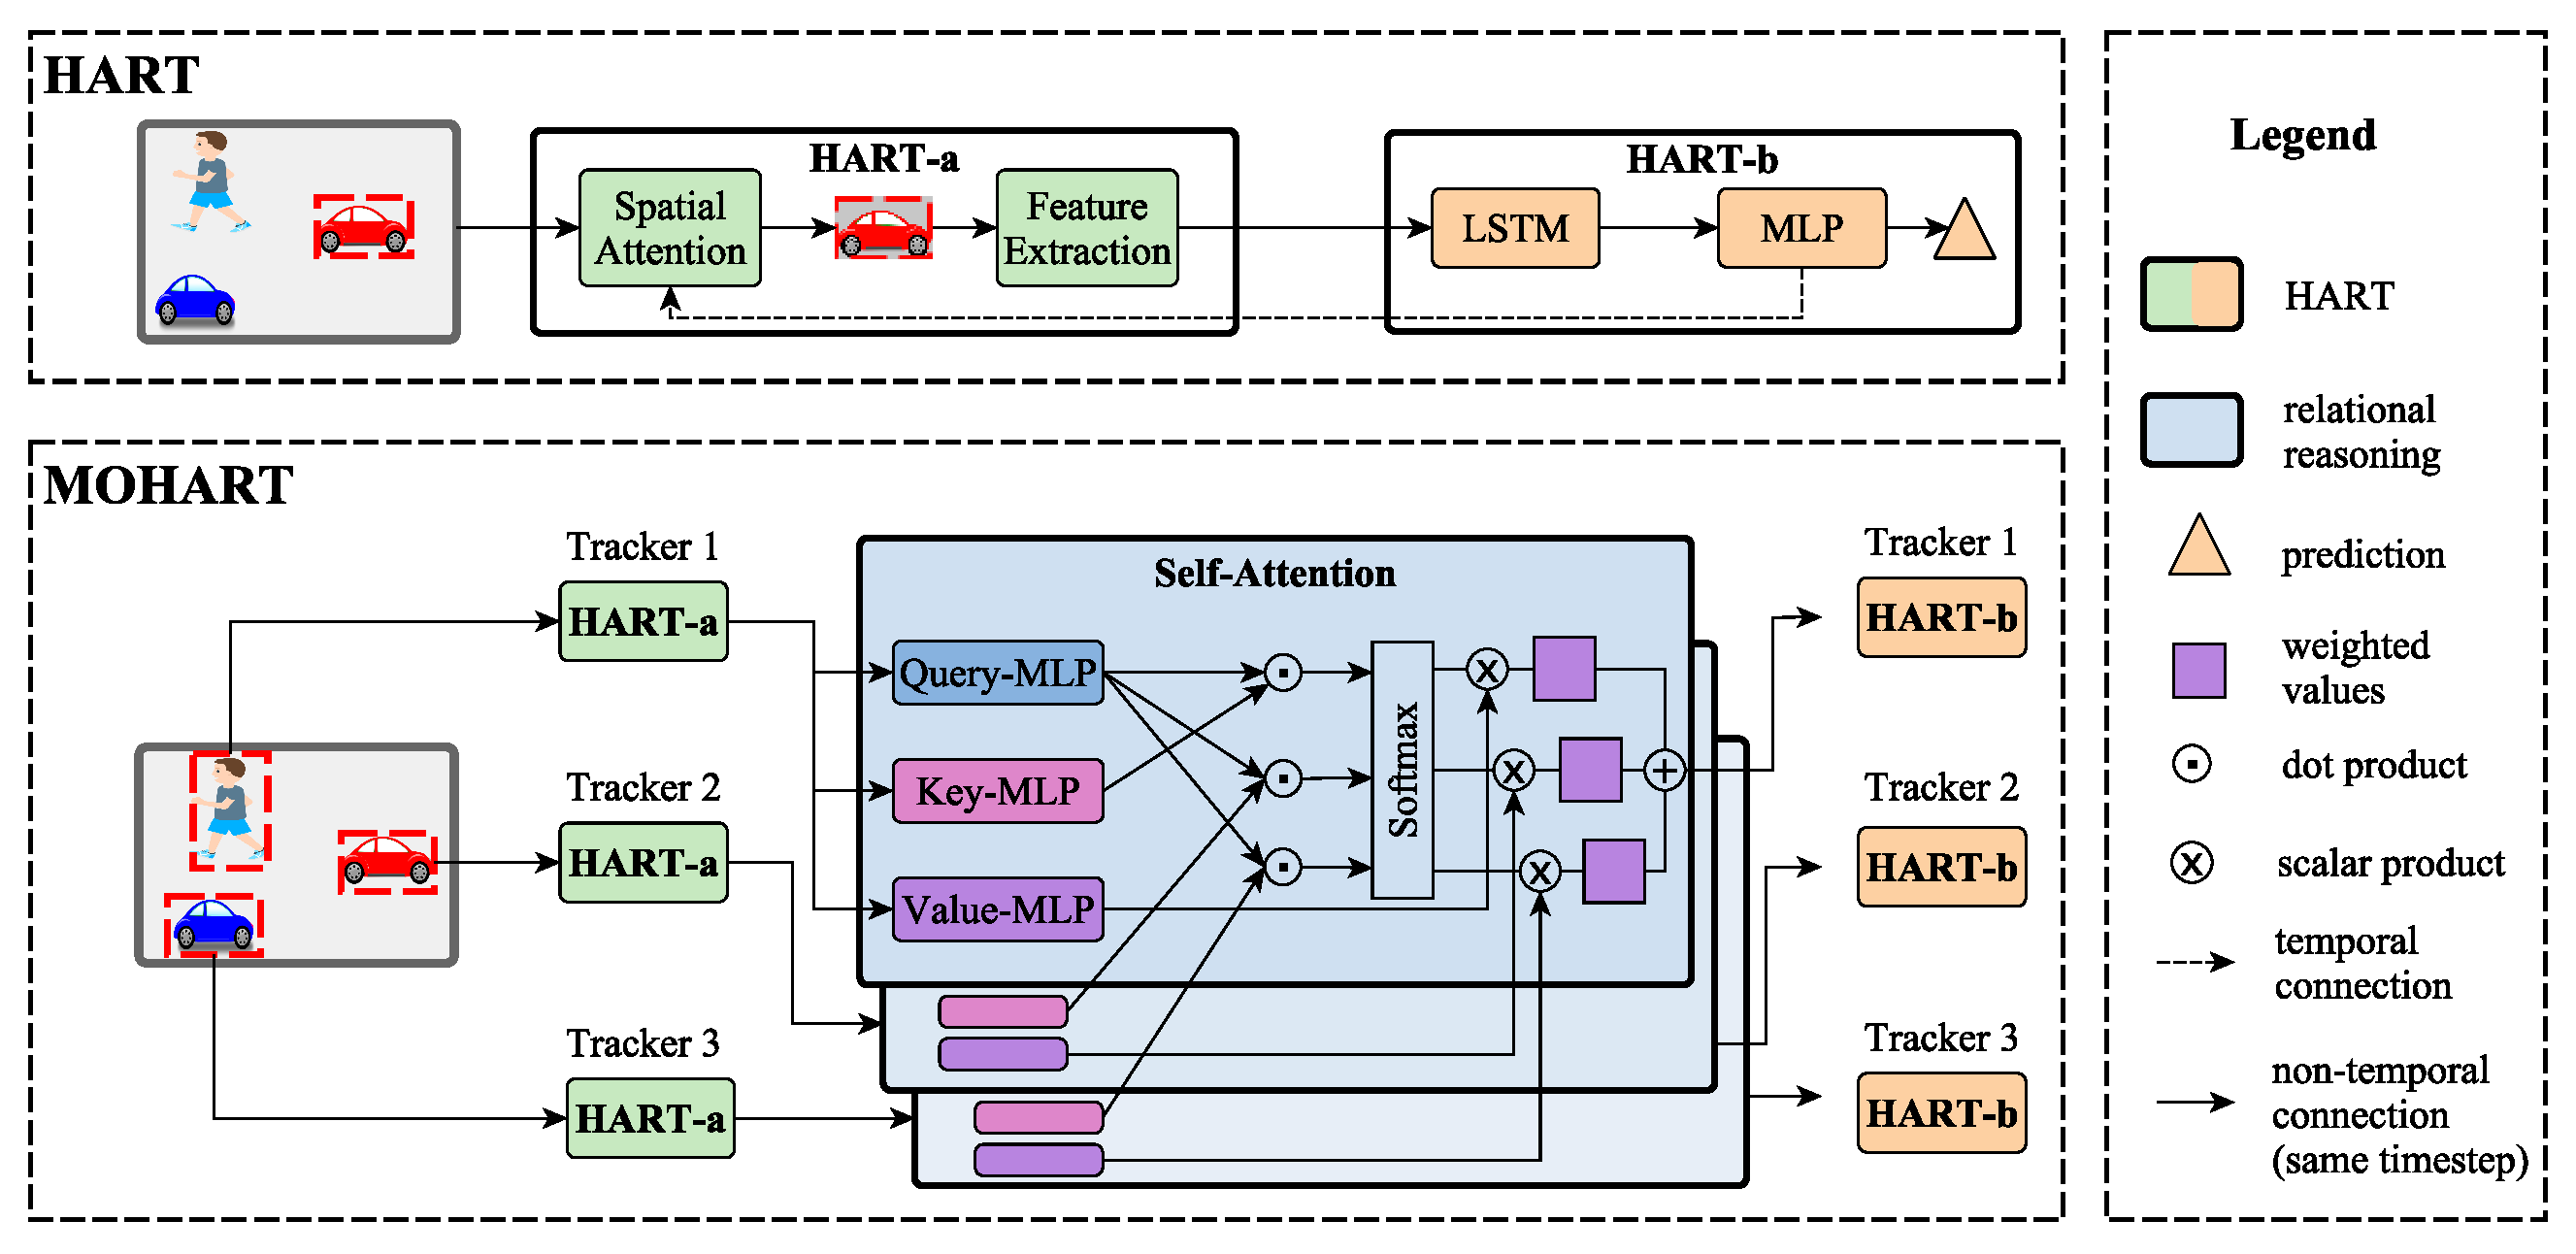
\includegraphics[width=1.0\textwidth]{figures/MOHART/system_large.pdf}
	\caption{Single-object tracking with \gls{HART} (top) and our extension to multi-object tracking (\gls{MOHART}, bottom). 
	We track multiple objects in a scene by applying multiple \gls{HART} trackers in parallel. 
	The trackers can exchange information about their respective objects using query-key-value attention.
	To do so, \gls{HART} is split into \gls{HART}-a and \gls{HART}-b (see top row) and we apply the self-attention mechanism in-between the parts.}
	\label{fig:system_large}
\end{figure}

We start by describing the \glsreset{HART}\gls{HART} algorithm \cite{Kosiorek17}, and then follow with an extension of \gls{HART} to tracking multiple objects, where multiple instances of \gls{HART} communicate with each other using multi-headed attention to facilitate relational reasoning. We also explain how this method can be extended to trajectory prediction instead of just tracking. 

\paragraph{Hierarchical Attentive Recurrent Tracking (\textsc{hart})}
\textsc{Hart} is an attention-based recurrent algorithm, which can efficiently track single objects in a video.
It uses a spatial attention mechanism to extract a \textit{glimpse} $\bg_t$, which corresponds to a small crop of the image $\bxt$ at time-step $t$, containing the object of interest.
This allows it to dispense with the processing of the whole image and can significantly decrease the amount of computation required.
\Gls{HART} uses a \gls{CNN} to convert the glimpse $\bg_t$ into features $\mathbf{f}_t$, which then update the hidden state $\mathbf{h}_t$ of a \gls{LSTM} core.
The hidden state is used to estimate the current bounding-box $\mathbf{b}_t$, spatial attention parameters for the next time-step $\ba_{t+1}$, as well as object appearance.
Importantly, the recurrent core can learn to predict complicated motion conditioned on the past history of the tracked object, which leads to relatively small attention glimpses---contrary to \gls{CNN}-based approaches \citep{Held2016goturn,Valmadre2017corr}, \gls{HART} does not need to analyse large regions-of-interest to search for tracked objects.
In the original paper, \textsc{hart} processes the glimpse with an additional ventral and dorsal stream on top of the feature extractor. Early experiments have shown that this does not improve performance on the MOTChallenge dataset, presumably due to the oftentimes small objects and overall small amount of training data. 
\Cref{fig:system_large} illustrates \gls{HART}, further details are provided in \Cref{sec:architecture_details}.

	The algorithm is initialised with a bounding-box\footnote{We can use either a ground-truth bounding-box or one provided by an external detector; the only requirement is that it contains the object of interest.} $\mathbf{b}_1$ for the first time-step, and operates on a sequence of raw images $\bx_{1:T}$.
	For time-steps $t\geq2$, it recursively outputs bounding-box estimates for the current time-step and predicted attention parameters for the next time-step. The performance of both algorithms is measured as intersection-over-union (IoU) averaged over all time steps in which an object is present, excluding the first time step.

Although \gls{HART} can track arbitrary objects, it is limited to tracking one object at a time.
While it can  be deployed on several objects in parallel, different \gls{HART} instances have no means of communication.
This results in performance loss, as it is more difficult to identify 
occlusions, ego-motion and object interactions.
Below, we propose an extension of \gls{HART} which remedies these shortcomings.

\paragraph{Multi-Object Hierarchical Attentive Recurrent Tracking (\textsc{mohart})}
Multi-object support in \gls{HART} requires the following modifications.
Firstly, in order to handle a dynamically changing number of objects, we apply \gls{HART} to multiple objects in parallel, where all parameters between \gls{HART} instances are shared. 
We refer to each \gls{HART} instance as a \textit{tracker}.
Secondly, we introduce a presence variable $p_{t,m}$ for object $m$.
It is used to mark whether an object should interact with other objects, as well as to mask the loss function (described in \cite{Kosiorek17}) for the given object when it is not present.
In this setup, parallel trackers cannot exchange information and are conceptually still single-object trackers, which we use as a baseline, referred to as \gls{HART} (despite it being an extension of the original algorithm).
Finally, to facilitate communication between trackers, we augment \gls{HART} with an additional step between feature extraction and the \gls{LSTM}.

Let $\mathbf{f}_{t, m}$ be the feature vector extracted from the glimpse corresponding to the m$^\mathrm{th}$ object, and let $\mathbf{f}_{t, 1:M}$ be the set of such features extracted from all glimpses.
Since different objects can interact with each other, it is necessary to use a method that can inform each object about the effects of their interactions with other objects.
Moreover, since features extracted from different objects comprise a set, this method should be permutation-equivariant,\ie the results should not depend on the order in which object features are processed.
Therefore, we use the multi-head self-attention block (\textsc{sab}, \citet{Lee2019settransformer}), which is able to account for higher-order interactions between set elements when computing their representations, thereby allowing rich information exchange, and it can do so in a permutation-equivariant manner.
Intuitively, in our case, \textsc{sab} allows any of the trackers to query other trackers about attributes of their respective objects,\eg distance between objects, their direction of movement, or their relation to the robot.
This is implemented as follows,
\begin{align}
Q &= W_q \mathbf{f}_{1:M} + b_q\,, \qquad K = W_k \mathbf{f}_{1:M} + b_k\,, \qquad V = W_v \mathbf{f}_{1:M} + b_v \label{eq:projection}\,,\\
&\hspace{1.5em} O_i = \operatorname{softmax}\left( Q_i K_i^T \right) V_i\,, \qquad i=1,\dots,H\,, \label{eq:att}\\
&\hspace{7em} o_{1:M} = O = \operatorname{concat}(O_i,\dots,O_H)\,, \label{eq:multihead}
\end{align}
where $o_m$ is the output of the relational reasoning module for object $m$. Time-step subscripts are dropped to decrease clutter.
In \Cref{eq:projection}, each of the extracted features $\mathbf{f}_{t,m}$ is linearly projected into a triplet of key $\mathbf{k}_{t,m}$, query $\mathbf{q}_{t,m}$ and value $\mathbf{v}_{t,m}$ vectors. Together, they comprise $K, Q$ and $V$ matrices with $M$ rows and $d_q, d_k, d_k$ columns, respectively.
$K, Q$ and $V$ are then split up into multiple heads $H \in \mathbb{N}_+$, which allows to query different attributes by comparing and aggregating different projection of features.
Multiplying $Q_iK_i^T$ in \Cref{eq:att} allows to compare every query vector $\mathbf{q}_{t,m,i}$ to all key vectors $\mathbf{k}_{t,1:M,i}$, where the value of the corresponding dot-products represents the degree of similarity.
Similarities are then normalised via a $\operatorname{softmax}$ operation and used to aggregate values $V$.
Finally, outputs of different attention heads are concatenated in \Cref{eq:multihead}.
\textsc{Sab} produces $M$ output vectors, one for each input, which are then concatenated with corresponding inputs and fed into separate \gls{LSTM}s for further processing, as in \gls{HART}---see \Cref{fig:system_large}.

\Gls{MOHART} is trained fully end-to-end, contrary to other tracking approaches \cite{Zhang2008,Milan2014,Bae2017confidence,Keuper2018motion}.
It maintains a hidden state, which can contain information about the object's motion. One benefit is that in order to predict future trajectories, one can simply feed black frames into the model. Our experiments show that the model learns to fall back on the motion model captured by the \gls{LSTM} in this case. 



\section{Validation on Simulated Data} %Toy Example
\label{sec:experiment_toy}
%\vspace{-3mm}

%

%    	A scenario with random identity switches renders relational reasoning necessary for accurate prediction of location in next time step. Circles of the same colour repel each other, circles of different colours attract each other. The colour coded identities are randomly assigned in each time step rendering information exchange between trackers (i.e. relational reasoning) necessary. While \textsc{hart} (top, $46\%$ IoU) clearly struggles in this stochastic environment, \textsc{mohart} (bottom, $76\%$ IoU) predicts the future locations much more accurately. The numbers in the bottom row indicate the self-attention weights from the perspective of the top left tracker (yellow number box).
%    	\textsc{hart} (top, $46\%$ IoU) vs. \textsc{mohart} (bottom, $76\%$ IoU). Dashed lines show spatial attention, solid lines show predicted bounding boxes, faded circles indicate future ground truth locations. Circles of the same colour repel each other, circles of different colours attract each other. The colour coded identities are randomly assigned in each time step rendering information exchange between trackers (i.e. relational reasoning) necessary. The numbers in the bottom row indicate the self-attention weights from the perspective of the top left tracker (yellow number box).

We test and compare the relational reasoning capabilities of the proposed algorithms on a toy domain. The domain is a 2D squared box which contains circular objects with approximated elastic collisions (energy and momentum conservation) between objects and with walls. To investigate how the model understands motion patterns and interactions between objects, we train it to predict future object locations in contrast to traditional tracking.

In the first experiment, each circle exerts repulsive forces on each other, where the force scales with $1/r$, $r$ being the distance between them. Predicting the future location just using the previous motion of one object (i.e. without relational reasoning) accurately is therefore challenging. We show that \textsc{hart} as an end-to-end single-object tracker is able to capture complex motion patterns and leverage these to make accurate predictions (see \Cref{sec:appendix_toy}). This indicates that \textsc{hart} is able to draw conclusions about the (deterministic, but not static) force field.

%In the first scenario (\Cref{fig:toy1}), four circles each exert repulsive forces on each other, where the force scales with $1/r$, $r$ being their distance. \textsc{hart} is applied four times in parallel and is trained to predict the location of each circle three time steps into the future. The different forces from different objects lead to a non-trivial force field at each time step. Predicting the future location just using the previous motion of one object (\Cref{fig:toy1} shows that each spatial attention box covers only the current object) accurately is therefore challenging. Surprisingly, the single object tracker solves this task with an average of $95\%$ IoU over sequences of 15 time steps. This shows the efficacy of end-to-end tracking to capture complex motion patterns and use them to predict future locations. This, of course, could also be used to generate robust bounding boxes for a tracking task.

\begin{figure}
    \centering
    \begin{subfigure}[c]{0.49\linewidth}
        \centering
        \includegraphics[width=\linewidth]{figures/MOHART/toy_iou_over_timesteps.pdf}
    \end{subfigure}
    \begin{subfigure}[c]{0.49\linewidth}
        \centering
        \includegraphics[width=\linewidth]{figures/MOHART/dial.pdf}
    \end{subfigure}
    \vspace{-2mm}
    \caption{
        Left: average IoU over sequence length for different implementations of relational reasoning on the toy domain shown in \cref{fig:toy2} ($\text{randomness} = 1.0$). Right: performance depending on how often agents are re-assigned identities randomly (sequence length 15). The higher the randomness, the less static the force field is and the more vital relational reasoning is. For $\text{randomness} = 0.0$, identities still have to be reassigned in some cases in order to prevent deadlocks, this leads to a performance loss for all models, which explains lower performance of self-attention for $\text{randomness} = 0.0$.
        \vspace{-4mm}
    }
    \label{fig:toy_quant}
\end{figure}

In the second experiment, we introduce randomness, rendering the scenario not solvable for a single object tracker as it requires knowledge about the state of the other objects and relational reasoning (see \cref{fig:toy2}). In each time step, we assign a colour-coded identity to the objects. Objects of the same identity repel each other, object of different identities attract each other (the objects can be thought of as electrons and protons). The qualitative results in \cref{fig:toy2} show that \textsc{mohart}, using self-attention for relational reasoning, is able to capture these interactions with high accuracy.
\Cref{fig:toy_quant} (left) shows a quantitative comparison of augmenting \textsc{hart} with different relational reasoning modules when identities are re-assigned in every timestep ($\text{randomness} = 1.0$). Exchanging information between trackers of different objects in the latent space with an MLP leads to slightly worse performance than the \textsc{HART} baseline, while simple max-pooling performs significantly better ($\Delta \text{IoU} \sim 17\%$). This can be explained through the permutation invariance of the problem: the list of latent representation of the different objects has no meaningful order and the output of the model should therefore be invariant to the ordering of the objects. The MLP is in itself not permutation invariant and therefore prone to overfit to the (meaningless) order of the objects in the training data. Max-pooling, however, is permutation invariant and can in theory, despite its simplicity, be used to approximate any permutation invariant function given a sufficiently large latent space \citep{Wagstaff2019}. Max-pooling is often used to exchange information between different tracklets, e.g., in the trajectory prediction domain \citep{Alahi2016social,Gupta2019social}. However, self-attention, allowing for learned querying and encoding of information, solves the relational reasoning task significantly more accurately. In \cref{fig:toy_quant} (right), the frequency with which object identities are reassigned randomly is varied. The results show that, in a deterministic environment, tracking does not necessarily profit from relational reasoning - even in the presence of long-range interactions. The less random, the more static the force field is and a static force field can be inferred from a small number of observations (see \cref{fig:toy1}). This does not mean that all stochastic environments profit from relational reasoning. What these experiments indicate is that tracking can not be expected to profit from relational reasoning by default in any environment, but instead in environments which feature (potentially non-deterministic) dynamics and predictable interactions.
\section{Relational Reasoning in Real-World Tracking}
%\vspace{-3mm}
\label{sec:experiment_real}

\begin{figure}[t!]
	\centering
	\includegraphics[width=1.0\textwidth]{figures/MOHART/mot_example2.png}
	\vspace{-6mm}
	\caption{Camera blackout experiment on a street scene from the MOTChallenge dataset with strong ego-motion. Solid boxes are \textsc{mohart} predictions (for $t\geq 2$), faded bounding boxes indicate object locations in the first frame. As the model is trained end-to-end, \textsc{mohart} learns to fall back onto its internal motion model if no new observations are available (black frames). As soon as new observations come in, the model 'snaps' back onto the tracked objects.}
	\label{fig:blackout_main}
\end{figure}

Having established that \textsc{mohart} is capable of performing complex relational reasoning, we now test the algorithm on three real world datasets and analyse the effects of relational reasoning on performance depending on dataset and task. We find consistent improvements of \textsc{mohart} compared to \textsc{hart} throughout. Relational reasoning yields particularly high gains for scenes with ego-motion, crowded scenes, and simulated faulty sensor inputs.

\subsection{Experimental Details}
\label{sec:exp_details}

We investigate three qualitatively  different datasets: the MOTChallenge dataset \citep{Mot16}, the UA-DETRAC dataset \citep{Wen15}, and the Stanford Drone dataset \citep{Dronedataset}. To increase scene dynamics and make the tracking/prediction problems more challenging, we sub-sample some of the high framerate scenes with a stride of two, resulting in scenes with 7-15 frames per second. Training and architecture details are given in \Cref{sec:mohart_experimental_details,sec:mohart_architecture_details}.
We conduct experiments in three different modes:


\textbf{Tracking.} The model is initialised with the ground truth bounding boxes for a set of objects in the first frame. It then consecutively sees the following frames and predicts the bounding boxes. The sequence length is 30 time steps and the performance is measured as intersection over union (IoU) averaged over the entire sequence excluding the first frame. This algorithm is either applied to the entire dataset or subsets of it to study the influence of certain properties of the data.

\textbf{Camera Blackout.} This simulates unsteady or faulty sensor inputs. The setup is the same as in 
\textit{Tracking}, but sub-sequences of the input are replaced with black images. The algorithm is expected to recognise that no new information is available and that it should resort to its internal motion model.

\textbf{Prediction.} Testing \textsc{mohart}'s ability to capture motion patterns, only the first two frames are shown to the model followed by three black frames. IoU is measured seperately for each time step.



\begin{table}[!ht]

{\footnotesize

  \floatsetup{floatrowsep=qquad, captionskip=4pt}
        \ttabbox%
    {\begin{tabularx}{\textwidth}{l*{5}{>{\raggedleft\arraybackslash}X}}
      \toprule
&                   Entire &            Only &              No  &               Crowded &           Camera \\%[-0.4em]
&                   Dataset &           Ego-Motion &        Ego-Motion &        Scenes &            Blackout \\
      \midrule
\textbf{MOHART} &   \textbf{68.5\%} &   \textbf{66.9\%} &   \textbf{64.7\%} &   \textbf{69.1\%} &   \textbf{63.6\%}  \\[0.1em]
HART &              66.6\% &            64.0\% &            62.9\% &            66.9\% &            60.6\%  \\
\midrule
$\Delta$ &          1.9\% &             2.9\% &             1.8\% &             2.2\% &             3.0\%  \\ 
\bottomrule
      \addlinespace
      \addlinespace
      \addlinespace
      \end{tabularx}}
    {\caption{Tracking performance on the MOTChallenge dataset measured in IoU.}
      \label{tab:results_motc}}
  \begin{floatrow}[2]

      
    \ttabbox%
    {\begin{tabularx}{0.55\textwidth}{l*{3}{>{\raggedleft\arraybackslash}X}}
      \toprule
      & All & Crowded Scenes & Camera Blackout \\
      \midrule
      \textbf{MOHART} & 68.1\% & \textbf{69.5\%} & \textbf{64.2\%}\\
      [0.1em]
      HART & \textbf{68.4\%} & 68.6\% & 53.8\%\\
      \midrule
      $\Delta$ & -0.3\% & 0.9\% & 0.4\%\\
      \bottomrule
      \end{tabularx}}
    {\caption{UA-DETRAC Dataset}
      \label{tab:results_detrac}}
    \hfill%
    \ttabbox%
    {\begin{tabularx}{0.35\textwidth}{r*{3}{>{\raggedleft\arraybackslash}X}}
      \toprule
      All & Camera Blackout & CamBlack Bikes \\
      \midrule
      \textbf{57.3\%} & \textbf{53.3}\% & \textbf{53.3\%} \\
      [0.1em]
      56.1\% & 52.6\% & 50.7\%\\
      \midrule
      1.2\% & 0.7\% & 2.6\%\\
      \bottomrule
      \end{tabularx}}
    {\caption{Stanford Drone Dataset}
      \label{tab:results_stanford}}
  \end{floatrow}
  
  }
\end{table}%



\subsection{Results and Analysis}


On the MOTChallenge dataset, \textsc{hart} achieves $66.6\%$ intersection over union (see \Cref{tab:results_motc}), which in itself is impressive given the small amount of training data of only 5225 training frames and no pre-training. \textsc{mohart} achieves $68.5\%$ (both numbers are averaged over 5 runs, independent samples $t$-test resulted in $p < 0.0001$). The performance gain increases when only considering ego-motion data. This is readily explained: movements of objects in the image space due to ego-motion are correlated and can therefore be better understood when combining information from movements of multiple objects, i.e. performing relational reasoning. In another ablation, we filtered for only crowded scenes by requesting five objects to be present for, on average, 90\% of the frames in a sub-sequence. For the MOT-Challenge dataset, this only leads to a minor increase of the performance gain of \textsc{mohart} indicating that the dataset exhibits a sufficient density of objects to learn interactions. The biggest benefit from relational reasoning can be observed in the \textit{camera blackout} experiments (setup explained in \Cref{sec:exp_details}). Both \textsc{hart} and \textsc{mohart} learn to rely on their internal motion models when confronted with black frames and propagate the bounding boxes according to the previous movement of the objects. It is unsurprising that this scenario profits particularly from relational reasoning. Qualitative tracking and \textit{camera blackout} results are shown in \cref{fig:blackout_main} and \Cref{sec:blackout}.

Tracking performance on the UA-DETRAC dataset only profits from relational reasoning when filtering for crowded scenes (see \Cref{tab:results_detrac}). The fact that the performance of \textsc{mohart} is slightly worse on the vanilla dataset ($\Delta = -0.3\%$) can be explained with more overfitting. As there is no exchange between trackers for each object, each object constitutes an independent training sample.

The Stanford drone dataset (see \Cref{tab:results_stanford}) is different to the other two---it is filmed from a birds-eye view.
The scenes are more crowded and each object covers a small number of pixels, rendering it a difficult problem for tracking.
The dataset was designed for trajectory prediction---a setup where an algorithm is typically provided with ground-truth tracklets in coordinate space and potentially an image as context information. The task is then to extrapolate these tracklets into the future. The tracking performance profits from relational reasoning more than on the UA-DETRAC dataset but less than on the MOTChallenge dataset. The performance gain on the \textit{camera blackout} experiments are particularly strong when only considering cyclists. 

In the \textit{prediction} experiments (see \Cref{sec:exp_pred}), \textsc{mohart} consistently outperforms \textsc{hart}. On both datasets, the model outperforms a baseline which uses momentum to linearly extrapolate the bounding boxes from the first two frames. This shows that even from just two frames, the model learns to capture motion models which are more complex than what could be observed from just the bounding boxes (i.e. momentum), suggesting that it uses visual information (\textsc{hart} \& \textsc{mohart}) as well as relational reasoning (\textsc{mohart}).

\section{Conclusion}
\label{sec:discussion}

With MOHART, we introduce an end-to-end multi-object tracker that is capable of capturing complex interactions and leveraging these for precise predictions as experiments both on toy and real world data show. However, the experiments also show that the benefit of relational reasoning strongly depends on the nature of the data. The toy experiments showed that in an entirely deterministic world relational reasoning was much less important than in a stochastic environment. Amongst the real-world dataset, the highest performance gains from relational reasoning were achieved on the MOTChallenge dataset, which features crowded scenes, ego-motion and occlusions.

\section*{Acknowledgements}
We thank Stefan Saftescu for his contributions, particularly for integrating the Stanford Drone Dataset, and Adam Golinski as well as Stefan Saftescu for proof-reading. This research was funded by the EPSRC AIMS Centre for Doctoral Training at Oxford University and an EPSRC Programme Grant (EP/M019918/1).
We acknowledge use of Hartree Centre resources in this work. The STFC Hartree Centre is a research collaboratory in association with IBM providing High Performance Computing platforms funded by the UK's investment in e-Infrastructure. The Centre aims to develop and demonstrate next generation software, optimised to take advantage of the move towards exa-scale computing.
{
\small
\bibliographystyle{plainnat}
\newpage\bibliography{main.bib}  % .bib
}
\newpage\clearpage
\appendix



\section{Experimental Details}
\label{sec:mohart_experimental_details}
The MOTChallenge and the UA-DETRAC dataset discussed in this section are intended to be used as a benchmark suite for multi-object-tracking in a tracking-by-detection paradigm. Therefore, ground truth bounding boxes are only available for the training datasets. The user is encouraged to upload their model which performs tracking in a data association paradigm leveraging the provided bounding box proposals from an external object detector. As we are interested in a different analysis (IoU given inital bounding boxes), we divide the training data further into training and test sequences. To make up for the smaller training data, we extend the MOTChallenge 2017 dataset with three sequences from the 2015 dataset (ETH-Sunnyday, PETS09-S2L1, ETH-Bahnhof). We use the first 70\% of the frames of each of the ten sequences for training and the rest for testing. Sequences with high frame rates (30Hz) are sub-sampled with a stride of two. For the UA-DETRAC dataset, we split the 60 available sequences into 44 training sequences and 16 test sequences. For the considerably larger Stanford Drone dataset we took three videos of the scene \textit{deathCircle} for training and the remaining two videos from the same scene for testing. The videos of the drone dataset were also sub-sampled with a stride of two to increase scene dynamics.


\section{Architecture Details}
\label{sec:mohart_architecture_details}
The architecture details were chosen to optimise \textsc{hart} performance on the MOTChallenge dataset. They deviate from the original \textsc{hart} implementation (\Cref{ch:hart}) as follows: A presence variable predicts whether an object is in the scene and successfully tracked. This is trained with a binary cross entropy loss. The maximum number of objects to be tracked simultaneously was set to 5 for the UA-DETRAC and MOTChallenge dataset. For the more crowded Stanford drone dataset, this number was set to 10. The feature extractor is a three layer convolutional network with a kernel size of 5, a stride of 2 in the first and last layer, 32 channels in the first two layers, 64 channels in the last layer, ELU activations, and skip connections. This converts the initial $32 \times 32 \times 3$ glimpse into a $7 \times 7 \times 64$ feature representation. This is followed by a fully connected layer with a 128 dimensional output and an elu activation. The spatial attention parameters are linearly projected onto 128 dimensions and added to this feature representation serving as a positional encoding. The LSTM has a hidden state size of 128. The self-attention unit in \textsc{mohart} comprises linear projects the inputs to dimensionality 128 for each keys, queries and values. For the real-world experiments, in addition to the extracted features from the glimpse, the hidden states from the previous LSTM state are also fed as an input by concatinating them with the features. In all cases, the output of the attention module is concatenated to the input features of the respective object.

As an optimizer, we used RMSProp with momentum set to $0.9$ and learning rate $5*10^{-6}$. For the MOTChallenge dataset and the UA-DETRAC dataset, the models were trained for 100,000 iterations of batch size 10 and the reported IoU is exponentially smoothed over iterations to achieve lower variance. For the Stanford Drone dataset, the batch size was increased to 32, reducing time to convergence and hence model training to 50,000 iterations.

\section{Deterministic Toy Domain}
\label{sec:appendix_toy}


\begin{figure}%
	\centering
	\includegraphics[width=0.99\textwidth]{figures/MOHART/sot_protons.png}
% 	\vspace{-3mm}
	\caption{
		\textsc{hart} single object tracking applied four times in parallel and trained to predict the location of each circle three time steps into the future. Dashed lines indicate spatial attention, solid lines are predicted bounding boxes, faded circles show ground truth location at $T+3$. Each circle exerts repulsive forces on each other, where the force scales with $1/r$, $r$ being their distance.
	}
	\label{fig:toy1}
\end{figure} 
%    	\textsc{hart} single object tracking applied four times in parallel. Dashed lines indicate spatial attention, solid lines are predicted bounding boxes at time step $T+3$, faded circles show the ground truth location at $T+3$. A repulsive force acts between each object pair which scales with distance as $1/r$. There is no information exchange between the trackers and each tracker evidently only `attends' to its own object. The fact that the future location is predicted accurately (i.e., much better than linear extrapolation) indicates that \textsc{hart} is able to capture complex motion patterns essentially allowing to draw conclusions about the force field. Shown are consecutive time steps from left to right.

In our first experiment in the toy domain (\Cref{fig:toy1}), four circles each exert repulsive forces on each other, where the force scales with $1/r$, $r$ being their distance. \textsc{hart} is applied four times in parallel and is trained to predict the location of each circle three time steps into the future. The different forces from different objects lead to a non-trivial force field at each time step. Predicting the future location just using the previous motion of one object (\Cref{fig:toy1} shows that each spatial attention box covers only the current object) accurately is therefore challenging. Surprisingly, the single object tracker solves this task with an average of $95\%$ IoU over sequences of 15 time steps. This shows the efficacy of end-to-end tracking to capture complex motion patterns and use them to predict future locations. This, of course, could also be used to generate robust bounding boxes for a tracking task.
\section{Prediction Experiments}
\label{sec:exp_pred}

\begin{figure}
    \centering
    \begin{subfigure}[c]{0.99\linewidth}
        \centering
        \includegraphics[width=\linewidth]{figures/MOHART/prediction_motc2.png}
        \vspace{-6mm}
        \caption{Prediction results on the MOTChallenge dataset \cite{Mot16}.}
        \label{fig:MOTC_imgs}
    \end{subfigure}
    \vspace{2mm}
    \begin{subfigure}[c]{0.99\linewidth}
        \centering
        \includegraphics[width=\linewidth]{figures/MOHART/prediction_detrac2.png}
        \vspace{-6mm}
        \caption{Prediction results on the UA-DETRAC dataset (crowded scenes only) \cite{Wen15}.}
        \label{fig:Detrac_quant}
    \vspace{-5mm}
    \end{subfigure}
\caption{Peeking into the future. Only the first two frames are shown to the tracking algorithm followed by three black frames. \textsc{mohart} learns to fall back on its internal motion model when no observation (i.e. only a black frame) is available. The reported IoU scores show the performance for the respective frames 0, 1, 2, and 3 time steps into the future.
\label{fig:prediction}
}
\end{figure}

In the results from the \textit{prediction} experiments (see \Cref{fig:prediction}) \textsc{mohart} consistently outperforms \textsc{hart}. On both datasets, the model outperforms a baseline which uses momentum to linearly extrapolate the bounding boxes from the first two frames. This shows that even from just two frames, the model learns to capture motion models which are more complex than what could be observed from just the bounding boxes (i.e. momentum), suggesting that it uses visual information (\textsc{hart} \& \textsc{mohart}) as well as relational reasoning (\textsc{mohart}). The strong performance gain of \textsc{mohart} compared to \textsc{hart} on the UA-DETRAC dataset, despite the small differences for tracking on this dataset, can be explained as follows: this dataset features little interactions but strong correlations in motion. Hence when only having access to the first two frames, \textsc{mohart} profits from estimating the velocities of multiple cars simultaneously.
\section{Qualitative Tracking Results}
\label{sec:blackout}


\begin{figure}[ht!]
\centering
\includegraphics[width=1\textwidth]{figures/MOHART/tracking_qualitative.pdf}
\vspace{-8mm}
\caption{Tracking examples of both \textsc{hart} and \textsc{mohart}. Coloured boxes are bounding boxes predicted by the model, arrows point at challenging aspects of the scenes. (A) \& (C): Each person being tracked is temporarily occluded by a woman walking across the scene (blue arrows). \textsc{mohart}, which includes a relational reasoning module, handles this more robustly (compare red arrows).
\vspace{-4mm}}
\label{fig:tracking_and_predicting}
\end{figure}


%\appendix
\begin{figure}
	\centering
	\includegraphics[width=1.0\textwidth]{figures/MOHART/mot_example1.png}
	\vspace{-6mm}
	\caption{Camera blackout experiment on a pedestrian street scene from the MOTChallenge dataset without ego-motion. Subsequent frames are displayed going from top left to bottom right. Shown are the inputs to the model (some of them being black frames, i.e. arrays of zeroes) and bounding boxes predicted by \textsc{MOHART} (coloured boxes). This scene is particularly challenging as occlusion and missing sensor input coincide (fourth row).
		\vspace{-2mm}}
	\label{fig:blackout1}
\end{figure}

% \begin{figure}
% 	\centering
% 	\includegraphics[width=1.0\textwidth]{figures/MOHART/mot_example2.png}
% 	\vspace{-6mm}
% 	\caption{Camera blackout experiment on a street scene from the MOTChallenge dataset with strong ego-motion. The reader is encouraged to compare top left and bottom right frame to make the amount of ego-motion apparent.}
% 	\label{fig:blackout2}
% \end{figure}

In \Cref{sec:experiment_real}, we tested \textsc{mohart} on three different real world data sets and in a number of different setups. \Cref{fig:tracking_and_predicting} shows qualitative results both for \textsc{hart} and \textsc{mohart} on the MOTChallenge dataset.

Furthermore, we conducted a set of camera blackout experiments to test \textsc{mohart}'s capability of dealing with faulty sensor inputs. While traditional pipeline methods require careful consideration of different types of corner cases to properly handle erroneous sensor inputs, \textsc{mohart} is able to capture these automatically, especially when confronted with similar issues in the training scenarios. To simulate this, we replace subsequences of the images with black frames. \Cref{fig:blackout1} and \Cref{fig:blackout_main} show two such examples from the test data together with the model's prediction. \textsc{mohart} learns not to update its internal model when confronted with black frames and instead uses the LSTM to propagate the bounding boxes. When proper sensor input is available again, the model uses this to make a rapid adjustment to its predicted location and `snap' back onto the object. This works remarkably well in both the presence of occlusion (\Cref{fig:blackout1}) and ego-motion (\Cref{fig:blackout_main}). \Cref{tab:results_motc,tab:results_detrac,tab:results_stanford} show that the benefit of relational reasoning is particularly high in these scenarios specifically. These experiments can also be seen as a proof of concept of \textsc{mohart}'s capabalities of predicting future trajectories---and how this profits from relational reasoning.

\end{document}
